%!TEX root = ./BPM17.tex

\section{The Solution} % (fold)
\label{sec:our_approach}
%%%% CONTENT
% subsection 1: loops
% subsection 2: background K

% section our_approach (end)
%Our objective is to predict sequences of activities, by taking into account available a-priori knowledge, in a reasonable amount of time.
Predicting
%the next activity and the sequence of next activities of an ongoing case
the suffix of a given prefix is a problem that is tackled by state-of-the-art approaches that make use of LSTM-based RNNs~\cite{evermann,niek96732} (see section~\ref{subsec:RNNforpredictive} and~\ref{deeplearning-stateoftheart}).  We hence start from these approaches and build on top of them to take into account a-priori knowledge.


Before presenting our approach, we need to observe that a basic solution that can be used to leverage a-priori knowledge for making predictions is the one provided by the inclusion of the a-priori knowledge in the data used for training the prediction model.
%\todo{It is hard to say if it is the easiest to put in the training. It should actually be harder to put a-priori knowledge in training and expect 100 percent compliance on prediction time.}
However, this solution would raise a main practical problem: since the a-priori knowledge can in principle change from case to case, this would require to retrain the model for each prediction, thus hampering the scalability of the predictive system. A smarter approach is hence required for taking into account a-priori knowledge when predicting the future path of an ongoing case.

In the next sections, we first introduce an enhancement, called \nocycle, of state-of-the-art approaches for overcoming the issues encountered with traces characterized by a high number of cycles (Section~\ref{ssec:noloop}). We then describe a further extension that allows us to take into account a-priori knowledge expressed in terms of LTL rules (Section~\ref{ssec:apriori}). The extension algorithm for accounting for a-priori knowledge and the enhancement for dealing with cycles are then combined into the \protrack technique.

\subsection{Learning from Trace Structures}
\label{ssec:noloop}

By experimenting the LSTM approach on different event logs, we found that event logs with traces containing a high number of repetitions of cycles perform worse than others, as also observed in~\cite{niek96732}. This is mainly due to the fact that frequent repetitions of a cycle cause an increase in the probability distribution of the back-loop, i.e., the connection between the last and the first element of the cycle.
To overcome this problem, we propose to equip Algorithm~\ref{alg:baseline} with an additional function in charge of weakening such a back-loop probability. This function is composed of two parts: in the first part, the current trace is analyzed in order to discover possible cycles; in the second part, the cycle discovery is used for preventing the prediction of further repetitions of the cycle. %(and possibly getting stuck in the loop). %making harder for the model to predict a further repetition of the loop (and possibly get stuck in the loop).%weakening the weight that causes a new repetition of the loop.
More in detail:
\begin{enumerate}
\item For each prefix $p_k(\sigma)=\left\langle a_1a_2 \ldots a_k\right\rangle$ of size $k$, the algorithm checks if there are $j$ ($j>=2$) consecutive occurrences of a cycle $c=\left\langle a_{c_1}\ldots a_{c_s}\right\rangle$, such that the last activity of the prefix corresponds to the last activity of the cycle $idx(a_k)=idx(a_{c_s})$;
\item $j$ is then used to correct the distribution over different possible activities that can occur in the next position by decreasing the probability of the first activity of the cycle $a_{c_1}$ to occur again. To decrease this probability, the algorithm uses a coefficient, function of the number of cycle repetitions $j$, as a weight to adjust the probability distribution. Examples of formulas that can be used for this purpose are $j^{2}$ or $e^{j}$.
%The formula can change for different logs. \todocdf{What does it mean?} %We are using $e^{x}
%The formula chosen depends on the average number of cycles per trace in the corresponding log. For a bigger number of cycles, the more steep function is selected.
 %(for example $j^{2}$ or $e^{j}$) %, that is multiplying the output of the formula by the probability for the loop causing next event.
\end{enumerate}

In simple words the \nocycle technique looks for the current cycle. Figure~\ref{figure:nocycle1} shows how the inference algorithm would choose next event for prediction. Then figure~\ref{figure:nocycle2} shows how the algorithm without \nocycle technique would choose next event, even though the cycle is present. If the technique applied figure ~\ref{figure:nocycle3} shows that the probability to choose the event starting the cycle is diminished. After three times cycle is repeated~\ref{figure:nocycle4} the algorithm predict second most probable event, by this going out of the cycle.




\begin{figure}[!ht]
	\begin{center}  
		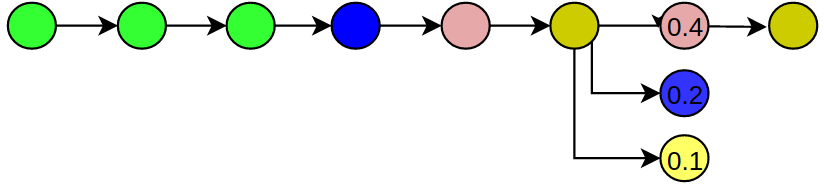
\includegraphics[scale=0.35]{nocycle-algo-1.png}
		\caption{How the next event is chosen}
		\label{figure:nocycle1}	
	\end{center}
\end{figure}

\begin{figure}[!ht]
	\begin{center}  
		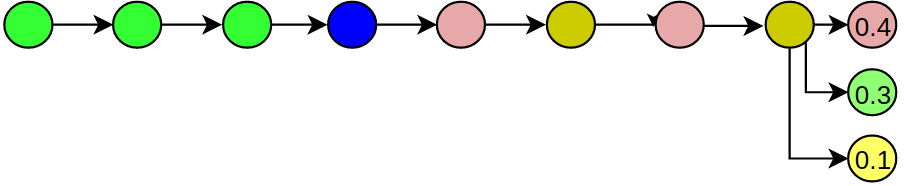
\includegraphics[scale=0.35]{nocycle-algo-2.png}
		\caption{How the next even standardly chosen (cycles present)}
		\label{figure:nocycle2}	
	\end{center}
\end{figure}

\begin{figure}[!ht]
	\begin{center}  
		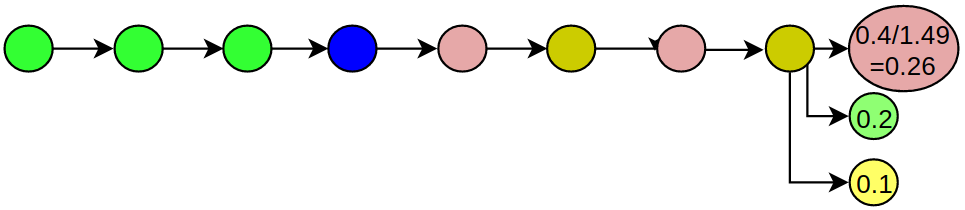
\includegraphics[scale=0.35]{nocycle-algo-3.png}
		\caption{Next event chosen after the $e^{2}$ applied for cycle size 2}
		\label{figure:nocycle3}	
	\end{center}
\end{figure}

\begin{figure}[!ht]
	\begin{center}  
		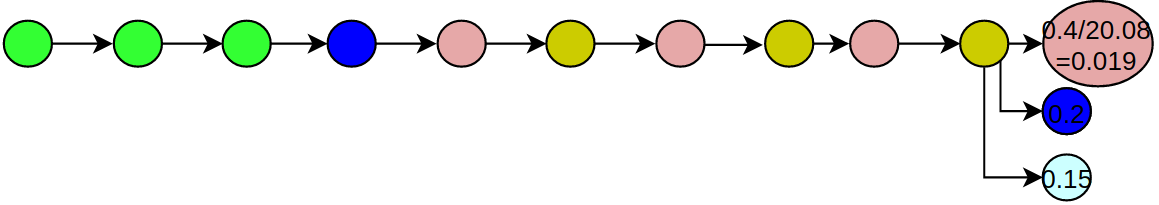
\includegraphics[scale=0.35]{nocycle-algo-4.png}
		\caption{Next event chosen after the $e^{2}$ applied for cycle size 3}
		\label{figure:nocycle4}	
	\end{center}
\end{figure}

Algorithm~\ref{alg:nocycle} reports the pseudo-code of the \nocycle technique. Similarly to Algorithm~\ref{alg:baseline} presented in Section~\ref{subsec:RNNforpredictive}, it takes as input a prefix $p_k(\sigma)$,  the trained LSTM model $lstm$, and the maximum number $max$ of iterations allowed. Then, it returns as output the complete trace (the prefix and the predicted suffix).  In particular, the algorithm adds to the state-of-the-art Algorithm~\ref{alg:baseline} the \textsc{weakenProb} procedure described above to find cycles in the trace and decrease the probability of the first activity of the cycle to occur again at the end of a repetition. The resulting vector of weakened probabilities is hence used for getting the next symbol as in the basic procedure.
%\todocdf{Remember to mention which formula we are using for the evaluation in the evaluation.}

\begin{algorithm}
%\scriptsize
	\caption{\nocycle extension for predicting the suffix of $p_k(\sigma)$}
	\begin{algorithmic}[1]
		\Function{PredictSuffixNoCycle}{$p_k(\sigma)$, $lstm$, $max$}
		\State $k$ = 0
		\State $trace$ = $p_k(\sigma)$
		\Do
		\State $trace_{encoded}$ = \textsc{encode}($trace$)
		\State $next\_symbol\_prob$ = \textsc{predictNextSymbols}($lstm$, $trace_{encoded}$)
		%\State $weakeaning\_coefficient$, $a_{c_1}$ = \textsc{computeWeakeningCoefficient}($trace$)
		\State $weak\_next\_symbol\_prob$ = \textsc{weakenProb} ($trace$, $next\_symbol\_prob$)
		\State $next\_symbol$ = \textsc{getSymbol}($weak\_next\_symbol\_prob$, $trace_{encoded}$)
		%\State $next\_symbol$ = getSymbolAmplified( $next\_symbol\_probabilities$ ,$amplifier$,$symbStartSycle$)
		\State $trace$ = $trace$ $\cdot$ $next\_symbol$
		\State $k$ = $k + 1$
		\doWhile{$($not $next\_symbol$ $==$ $end\_symbol)$ and $(k < max)$}
		\State \textbf{return} trace
		\EndFunction
		
%		\Function{amplify}{$trace$}
%	  \State $rep$ = findAllCycles($trace$)
%		\State \If{$rep$ contains curreny cycle in $trace$} {
%		\State numberOfRep = getNumberCurrentcycleRepeats($rep$,$trace$)
%		\State return amplifyFormula(numberOfRep), firstSymbolOfCurrentTrace}
%		\State return
%		\EndFunction

	%	\Function{getSymbolAmpl}{$nextSymbolProb$, $amplifier$,$symbStartSycle$}
	%	\State index = findItemIndex($symbStartSycle$)
	%	\State $nextSymbolProb$.item(index) = $nextSymbolProb$.item(index) * $amplifier$
	%	\State top = chooseMaxProb($nextSymbolProb$)
	%	\State return probabilityToSymbol(top)
	%	\EndFunction
	\end{algorithmic}
	\label{alg:nocycle}
\end{algorithm}


\subsection{Learning from A-priori Knowledge}
\label{ssec:apriori}

The overall idea for leveraging a-priori knowledge for predictive monitoring is simple: (i) we use the LSTM approach to get the possible predictions for an ongoing trace; this can be done, because the step by step output of a recurrent neural network is basically probability distribution over next events in the trace. (ii) we rank them according to the likelihood of the prediction; and (iii) we select the first prediction which is compliant with the LTL rules describing the a-priori knowledge. However, although RNN inference algorithms are not computationally expensive per se, building all the possible predicted suffixes could be costly and inefficient. It is the standard problem of algorithms that rely on storing data in tree structures, where the growth of a tree is exponential. That is exactly the case here, as nevertheless of how many continuation of the trace is chosen at each step (let's day $N$ steps), each next step of predictions will produce $N^{i}$ nodes. Even for few iterations it is computationally and memory-wise not feasible to use this strategy.

Therefore, the alternative investigated in this paper leverages, on top of state-of-the-art LSTM techniques, the approach classically used in statistical sequence-to-sequence predictions in translation tasks~\cite{Tillmann2003WRD778822778827}, i.e., the \textit{beamSearch} algorithm. The beamSearch works by the partial ordering of the probability trees, that is by exploring the search space, only taking the most promising branches.
In particular, we use the RNN architecture with LSTM cells and training system proposed in~\cite{niek96732}. Then, in the testing phase, to predict a certain suffix, we use a new inference algorithm (\protrack), which explores the probability space using beamSearch to cut the branches of the LSTM model which bring to predictions that are not compliant with the a-priori knowledge.
% (described in terms of LTL rules).

% The \protrack algorithm has been designed by modifying the inference Algorithm~\ref{alg:baseline} (presented in Section~\ref{sec:background}) to enable the breadth first beamSearch.
%For beamSearch we need to save the probability distribution over most probable of size of beam coefficient.
%\todocg{I've removed the sentence saying that protrack is built on top of \cite{niek96732} because it was already said two lines above.}
Algorithm~\ref{alg:protrack} reports the pseudo-code describing the \protrack algorithm. It takes as input the prefix $p_k(\sigma)$, the available a-priori knowledge $\cal{K}(\sigma)$, and the trained LSTM model $lstm$, together with three parameters: (i) $bSize$, which is the number of possible next symbols returned by the beamSearch algorithm; (ii) $maxSize$, which is the maximum number of branches that can be explored by \protrack at the same time; and (iii) $max$, which is the maximum number of allowed iterations.

\begin{algorithm}
	\caption{\protrack algorithm for predicting the suffix of $p_k(\sigma)$}
	\label{alg:protrack}
	\begin{algorithmic}[1]
		\Function{\protrack}{$p_k(\sigma)$, $\cal{K}(\sigma)$, $lstm$, $bSize$, $maxSize$, $max$}
		\State $h$ = 0
		\State $prefixes$ = \{$p_k(\sigma)$\}\label{lst2:initialization}
		\While {$k \leq max$ and not \textsc{empty}($prefixes$)} \label{lst2:while}
			\State $candidates\_next$ = \textsc{predictPrefNextSymbols}($lstm$, $prefixes$, $bSize$) \label{lst2:prediction}
			\State $top\_candidates$ = \textsc{topRank}$(candidates\_next$, $maxSize)$ \label{lst2:top}
			\ForAll {$candidate$ in $top\_candidates$} \label{lst2:forall}
%				\If {\textsc{check}$(candidate$, $\cal{K})$} \label{lst2:compliant}
				%	\State $trace$ = \textsc{predictSuffix}$(candidate)$ \label{lst2:predictsuffix}
			%		\State \textbf{return} $trace$
%				\Else
					\If {\textsc{last\_symbol}($candidate$) $<>$ $end\_symbol$}
						\State \textsc{push}($candidate$, $prefixes$)
\Else
					\If {\textsc{check}$(candidate$, $\cal{K})$} \label{lst2:compliant}
\State \textbf{return} $candidate$

\EndIf
				\EndIf
			\EndFor
			\State $h = h + 1$
		\EndWhile
		\EndFunction
	\end{algorithmic}
\end{algorithm}


%Intuitively, the algorithm iterates over a priority queue of prefixes, which is initialized with the input prefix $p_k$ (line~\ref{lst2:initialization}) and that is used for regulating the number of branches to be explored. At the first step, by leveraging the the $bSize$ next events are predicted for the prefix $p_k$ and $bSize$ new traces obtained by concatenating $p_k$ and each of the $bSize$ predicted next events

%If, at the first step, any of the prefixes of the queue is compliant to the formula, the next step consists of predicting for each prefix $p_k$ in $prefixes$ the $bSize$ next events and obtaining $bSize$ new traces by concatenating $p_k$ and each of the $bSize$ predicted next events. So, the algorithm will deal with $\|prefixes\|*bSize$ traces. However, in order to limit the search space, the algorithm ranks the predicted traces based on their estimated probability\footnote{Note that, in order to prevent overflow in the computation, the estimated probability for sequences of events is usually computed as the sum of the log probability (the logarithm of the probability) of the next events probability rather than as the product of the next events probability.} and only takes the top $maxSize$ traces.
%The algoirhtm is iterated until the queue is empty or the maximum number of iterations $max$ is reached (line \ref{lst2:prediction}).

%With this approach we limit our search space to a smaller one. This procedure is heuristic, so sometimes, with a beam size it is possible to cut out best, and/or compliant solutions. In real world testing it has been shown that even with beam size set to $3$, almost always the solutions are found.





\begin{figure}[!ht]
	\begin{center}  
		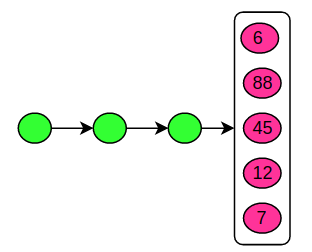
\includegraphics[scale=0.4]{beam-algo-1.png}
		\caption{Beam search based algorithm, step 1}
		\label{figure:beam1}	
	\end{center}
\end{figure}

\begin{figure}[!ht]
	\begin{center}  
		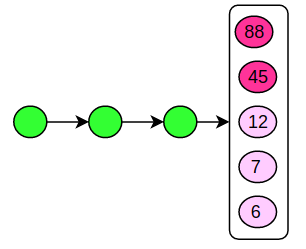
\includegraphics[scale=0.4]{beam-algo-2.png}
		\caption{Beam search based algorithm, step 2}
		\label{figure:beam2}	
	\end{center}
\end{figure}

\begin{figure}[!ht]
	\begin{center}  
		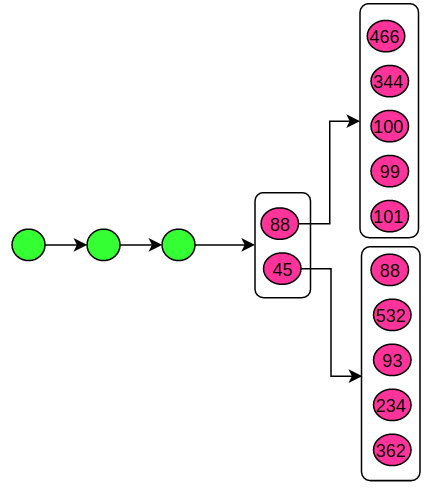
\includegraphics[scale=0.4]{beam-algo-3.png}
		\caption{Beam search based algorithm, step 3}
		\label{figure:beam3}	
	\end{center}
\end{figure}

\begin{figure}[!ht]
	\begin{center}  
		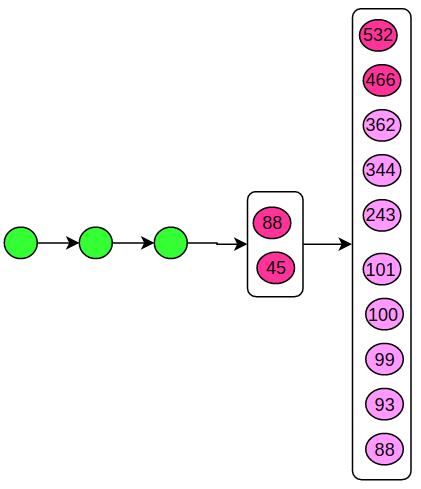
\includegraphics[scale=0.4]{beam-algo-4.png}
		\caption{Beam search based algorithm, step 4}
		\label{figure:beam4}	
	\end{center}
\end{figure}

To describe the algorithm we will use the graphics. The figure~\ref{figure:beam1} shows in green the prefix of the trace, and the pink are the 5 predicted next events. Their scores are displayed inside the circles. On the next step (figure~\ref{figure:beam2}), algorithm ranks the predicted events, and chooses $bSize$ traces (in the exemplary case it's 2). Next step (figure~\ref{figure:beam3}), is to predict next events for all possible traces saved. Then these traces are also ranked (figure~\ref{figure:beam4}) and next $bSize$ events are chosen. After the check on the LTL formula approves the predicted sequence, and end symbol is predicted, the process stops, and the sequence is returned (every node keeps a link to its parent node, so reconstruction of whole trace is not an issue).

Following pseudo code listing~\ref{alg:protrack}, the algorithm iterates over a priority queue of prefixes, which is initialized with the input prefix $p_k(\sigma)$ (line~\ref{lst2:initialization}) and that is used for regulating the number of branches to be explored. For each prefix in $prefixes$, $bSize$ ($< maxSize$) possible next activities are predicted (by means of the \textsc{predictNextSymbols} procedure of Algorithm~\ref{alg:baseline} and the beamSearch algorithm) and for each prefix $bSize$ new traces are obtained by concatenating the prefix with the corresponding $bSize$ predicted next activities (line 5). In this way, the algorithm generates $\left|prefixes\right|*bSize$ traces. In order to limit the search space, the algorithm ranks the predicted traces based on their estimated probability\footnote{Note that, in order to prevent overflow in the computation, the estimated probability for sequences of activities is computed as the sum of the logarithm of the probabilities of the next activities rather than as the product of the probabilities of the next activities.} and takes only the top $maxSize$ ones (line 6). For each of these traces (line 7), if the last symbol predicted is not the end symbol, the trace is added to $prefixes$ (line 9). Otherwise, if the trace is complete, the algorithm checks if it is compliant to the LTL rules in $\cal{K}(\sigma)$ (line 11). In this case, the trace is returned (line 12).
%In the next step, the procedure is iterated.
%the $bSize$ possible next activities are computed and $bSize$ new traces obtained, so that the algorithm will deal with $\left|prefixes\right|*bSize$ traces. At this point, in order to limit the search space, the algorithm ranks the predicted traces based on their estimated probability\footnote{Note that, in order to prevent overflow in the computation, the estimated probability for sequences of activities is computed as the sum of the logarithm of the probabilities of the next activities rather than as the product of the probabilities of the next activities.} and takes only the top $maxSize$ traces.
The algorithm is then iterated until the queue of prefixes is empty or the maximum number of iterations $max$ is reached (line 4).
%This procedure, although ensuring a reduced search space (limited to $maxSize$ nodes to be explored) is a heuristic procedure. Therefore, too low values of $bSize$ can possibly cut out good solutions.
%In real world settings, however, it has been shown that a $bSize$ of $3$ is sufficient to avoid this problem.








%The algorithm builds a priority queue of current prefixes, which at the first iteration only contains the prefix $p_k$ , and uses it as a priority queue for regulating the maximum number of branches to be explored that are active in parallel. It hence loops on such a structure until the queue $prefixes$ is empty or the maximum number of iterations $max$ is reached (line \ref{lst2:prediction}).
%The function \textsc{predictPrefixesNextSymbols} returns, by leveraging the \textsc{predictNextSymbols} procedure of Algorithm~\ref{alg:baseline} and the beam Search algorithm, for each prefix in the queue $prefixes$ of length $\hat{k}_i$, $biSize$ traces of length $\hat{k}_{i+1}$, obtained by concatenating $p_{\hat{k}}$ and the predicted next symbols. All the returned traces of length $\hat{k}_{i+1}$ are then ranked and only the top $maxSize$ are taken \ref{lst2:top}, to guarantee that not too many branches are explored in parallel. For each candidate trace, its compliance with respect to the a-priori knowledge  $\cal(K)$ is checked. If the trace is already compliant to $\cal{K}$, the predictSuffix procedure of Algorithm~\ref{alg:baseline} is invoked and the prediction returned, otherwise, if $p_{\hat{k}_{i+1}}$ has not yet reached the end symbol, the new prefix is added to the $prefixes$ priority queue.


%The algorithm first explores the N next activities given the prefix, and checks if any of them are compliant. If any of them are, the algorithm predicts the remaining trace to the end, assuming to be most probable. If on the first step the LTL formula compliant prefix not found, the next step consists of predicting for every N prefixes N next activities. So it will have $N*N$ resulting traces. The algorithm then decides to cut $N*N-N$ traces based on the estimated probability. It is done by summing up the log probability of the trace up to the last step.


\subsection{Implementation}
\label{ssec:implementation}
Algorithms~\ref{alg:nocycle} and~\ref{alg:protrack} have been implemented in Python 2.6. In particular, the Keras~\cite{chollet2015keras} and TensorFlow~\cite{tensorflow2015-whitepaper} libraries have been used for neural networks. The LTL checker~\cite{vanderAalst2005}\footnote{The LTL formula checker is taken from the open source code of ProM process mining suite.})for checking the compliance of traces to LTL rules is instead based on automata and written in Java~\cite{Westergaard2040296}. 

As the problem of compatibility arose having Java and Python parts, the Py4J library\cite{py4j} was used as a gateway to access Java code from Python.

The full source code is available on github\footnote{\url{https://github.com/yesanton/Process-Sequence-Prediction-with-A-priori-knowledge}}. The link given contain detailed readme with instruction on how to reproduce all experiments on any machine. 

%
%When building the \textit{first-best Beam search}, the tree structure was introduced that holds all necessary intermediate values, and up to N leaves. It stores the prefix up to now, parent node (for backtracking), the encoded data, total predicted time, and node status that can be discovered or closed.
%
%The node structure then used to save all path of predictions, and if the execution of the algorithm discovers that at the end the predicted trace is not compliant it starts backtracking to the first non closed node.
%
%For the breath first search the Queue class from Python library was used to store step-wise most probable outcomes.
%
%More implementation details can be seen on our github page.





%%% Local Variables:
%%% mode: latex
%%% TeX-master: "BPM17"
%%% End:
